\begin{surferPage}[%
משטח ממעלה שלישית 
]{%
משטח ממעלה שלישית של קיילי%
}
   זהו משטח ממעלה שלישית. הוא מופיע גם
    בגלריית המשטחים הפשוטים.
    הוא כולל ארבע נקודות סינגולריות כפולות-חרוט.
    המשטח נקרא על שם ארתור קיילי \textenglish{(Arthur Cayley)}
  שערך מספר גדול של מחקרים על משטחים מהמעלה השלישית
    במאה ה-$19$.

     ואולם, היה זה לוּדוויג שלַפלי
          \textenglish{(Ludwig Schl\"afli)}
          שבשנת 1863 סיווג לראשונה את המשטחים האלה
    בצורה שיטתית מבחינת מספר נקודות הסינגולריות שעליהם.
    לדוגמה, במאמר שכתב שלפלי באותה שנה תוכלו לקרוא מדוע לא יכולות להתקיים יותר מ-$4$
    נקודות סינגולריות על משטח מהמעלה השלישית.
    לפיכך: $\mu(3)=4$.

    בסביבות שנת 1900, חקר פליקס קליין
    \textenglish{(Felix Klein)}
     את הצורות האפשריות של משטחים אמתיים מהמעלה השלישית;
    כדי לענות על שאלה זו הוא התחיל במשטח מהמעלה השלישית של קיילי
    והכניס בו עיוותים קלים:
    הוא הרחיב נקודות סינגולריות כפולות חרוט, ניתק או חיבר חלקים שונים,
    ובדרך זו הצליח למצוא את כל הצורות האפשריות; הנה מספר דוגמאות:
    \vspace{0,3cm}
     \begin{center}
      \vspace{-0,2cm}
      \begin{tabular}{@{}c@{\ }c@{\ }c@{\ }c@{}}
        \begin{tabular}{@{}c@{}}
          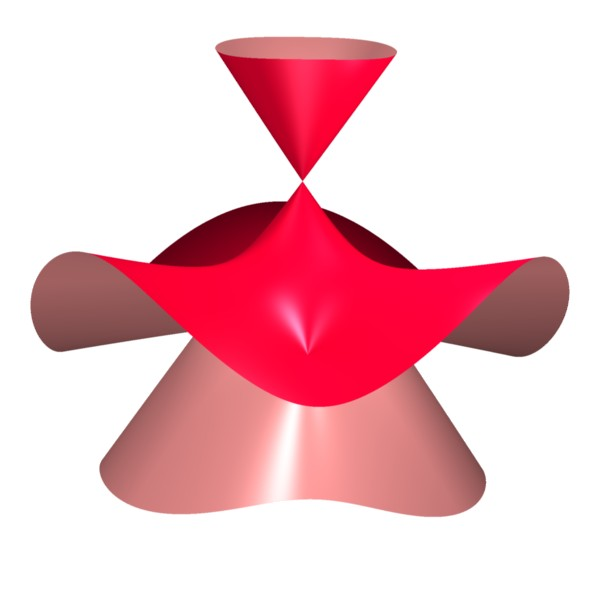
\includegraphics[width=1.35cm]{cayley_cubic_0}
        \end{tabular}
        &
        \begin{tabular}{@{}c@{}}
          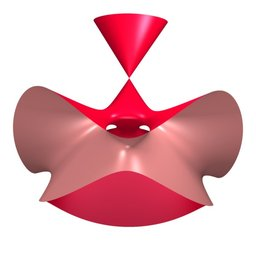
\includegraphics[width=1.35cm]{cayley_cubic_1}
        \end{tabular}
        &
        \begin{tabular}{@{}c@{}}
          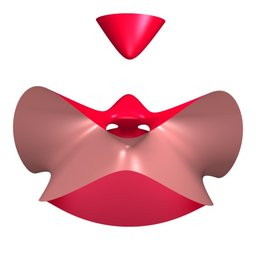
\includegraphics[width=1.35cm]{cayley_cubic_2}
        \end{tabular}
        &
        \begin{tabular}{@{}c@{}}
          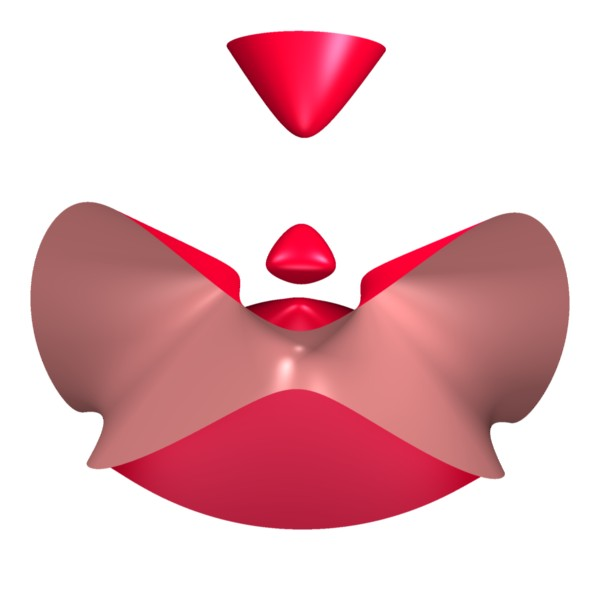
\includegraphics[width=1.35cm]{cayley_cubic_3}
        \end{tabular}
      \end{tabular}
    \end{center}
\end{surferPage}
